\documentclass[aspectratio=169]{beamer}

\usetheme{CambridgeUS}

\usepackage[utf8]{inputenc}
\usepackage[T1]{fontenc}
\usepackage{tikz}
\usepackage{pdfrender}
\usepackage{xcolor}
\usepackage[dvipsnames]{xcolor}
\definecolor{myblue}{RGB}{0, 0, 80}
\usepackage{array}
\usepackage[spanish,es-tabla]{babel}
\usetikzlibrary{shapes,arrows}
\selectlanguage{spanish}

%===========================Portada============================================
%==============================================================================
%==============================================================================
\title[]{Aplicación de Redes Neuronales Para Estimar la Ubicación\\ de Objetos Tridimensionales en Habitaciones Pequeñas \\Utilizando Ecos Acústicos}
\subtitle[]{Tesis de Maestría en Computación}
\author[]{Autor: Esteban Padilla Padilla\\Supervisor: Ing. Kervin Sánchez Herrera M.Sc.}
\institute[]{Escuela de Ingeniería en Computación\\Instituto Tecnológico de Costa Rica}
\date[]{27 Junio 2025}

\setbeamerfont{title}{size=\fontsize{15}{10}\bfseries}
\setbeamerfont{subtitle}{size=\fontsize{12}{10}\bfseries}
\setbeamerfont{author}{size=\fontsize{10}{10}\bfseries}
\setbeamerfont{institute}{size=\fontsize{10}{10}\bfseries}
\setbeamerfont{date}{size=\fontsize{8}{10}\bfseries}

%Formato Portada
\setbeamertemplate{title page}{%

    \begin{tikzpicture}[remember picture,overlay]
    
    %Imagen principal
    \node[anchor=south] at ([yshift=-0.15cm]current page.south) {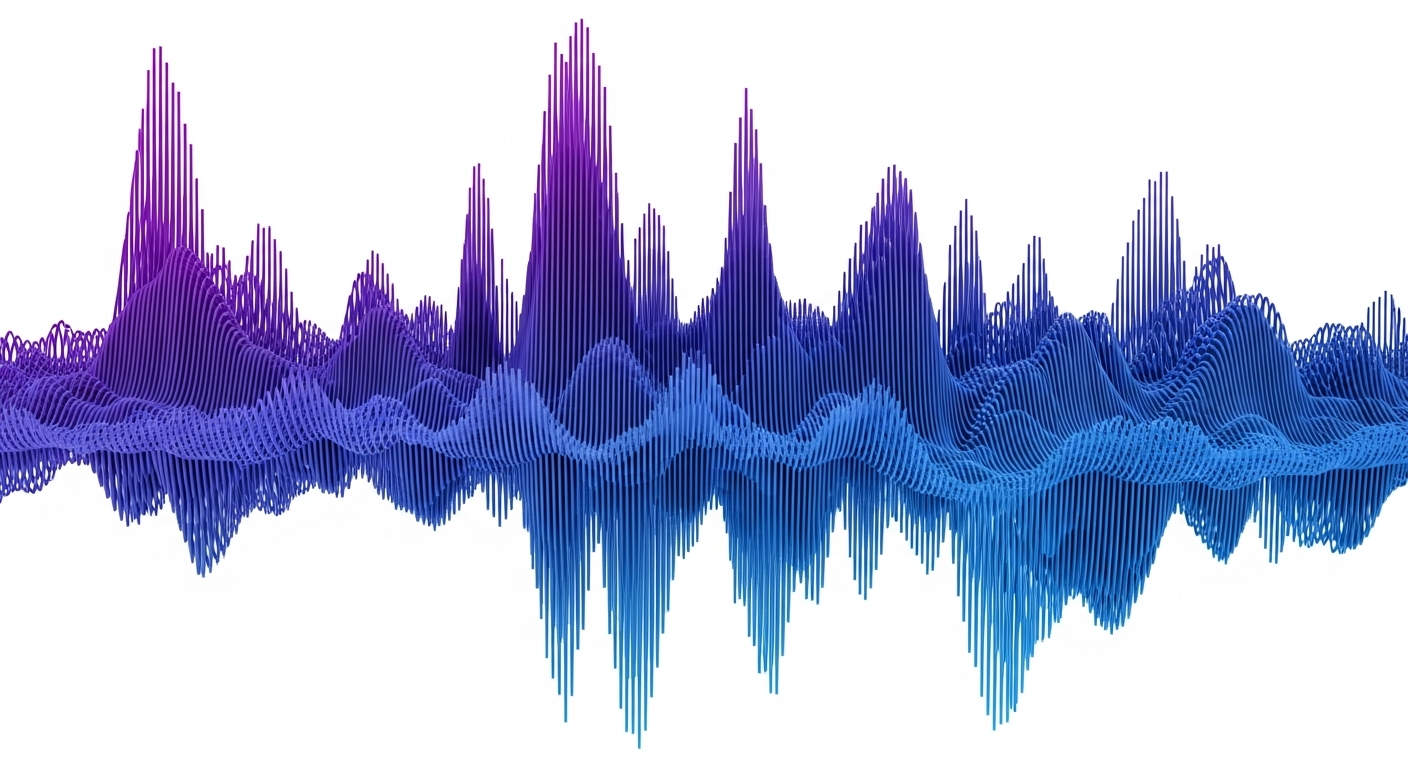
\includegraphics[width=\paperwidth,height=3cm]{Whisk_4529d9a66c.jpg}};
    
    %Titulo
    \node[anchor=east] at ([xshift=0pt, yshift=-50pt]current page.north east) (title)
    {\parbox[t]{\textwidth}{\centering%
            \usebeamerfont{title}\textcolor{black}{%
                \textpdfrender{}{\inserttitle}}}};
                
    %Sutitulo
    \node[anchor=east] at ([xshift=-80pt, yshift=-90pt] current page.north east) (subtitle)
    {\parbox[t]{.6\paperwidth}{\raggedleft%
            \usebeamerfont{subtitle}\textcolor{black}{%
                \textpdfrender{}{\insertsubtitle}}}};
    
    %Autor
    \node[anchor=east] at ([xshift=0pt, yshift=-115pt] current page.north east) (author)
    {\parbox[t]{\paperwidth}{\centering%
            \usebeamerfont{author}\textcolor{NavyBlue}{%
                \textpdfrender{}{\insertauthor}}}};
    
    %Instituto
    \node[anchor=east] at ([xshift=0pt, yshift=-140pt]current page.north east) (institute)
    {\parbox[t]{\paperwidth}{\centering%
            \usebeamerfont{institute}\textcolor{NavyBlue}{\insertinstitute}}};
    
    %Fecha
    \node[anchor=east] at ([xshift=-195pt,yshift=-165pt]current page.north east) (date)
    {\parbox[t]{.78\paperwidth}{\raggedleft%
            \usebeamerfont{date}\textcolor{black}{\insertdate}}};


    %Imagen titulo
    \node[anchor=south west] at ([xshift=-35pt,yshift=-10pt]current page.west) (logo)
    {\parbox[t]{.19\paperwidth}{\raggedleft%
            \usebeamercolor[fg]{titlegraphic}\inserttitlegraphic}};
    
    
    \end{tikzpicture}
}
\titlegraphic{
\includegraphics[width=1.8cm]{TEC}}
\setbeamertemplate{caption}[numbered]
%\usepackage[font=scriptsize,justification=centering]{caption}
\usepackage[justification=centering]{caption}

\begin{document}
    \begin{frame}[plain]
        \maketitle
    \end{frame}

%\beamerdefaultoverlayspecification{<+->}
\setbeamertemplate{page number in head/foot}{}
\setbeamercolor{itemize/enumerate body}{fg=gray}
\setbeamertemplate{navigation symbols}{}

%\begin{frame}{}

%¿Por qué concentrarse en la redacción de una tesis cuando el problema principal es la investigación?
        %\uncover<3->{
%        \begin{figure}
%        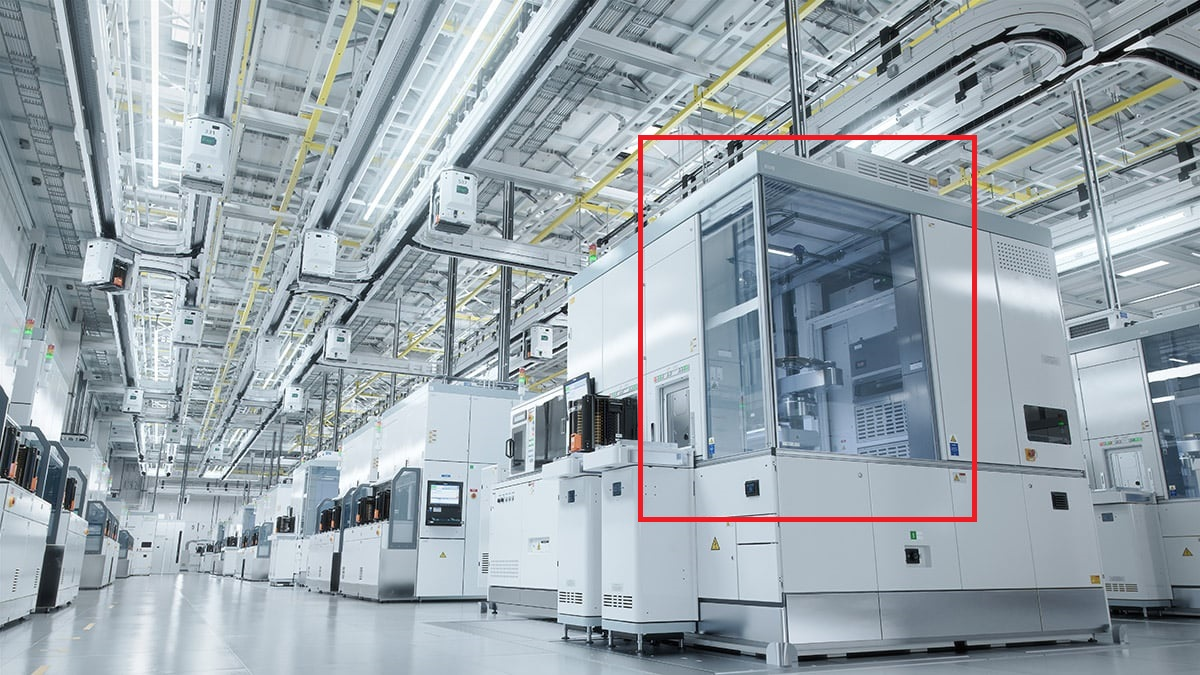
\includegraphics[width=15cm, height=8cm]{semiconductor-manufacturing-facility.jpg}
        %\caption{here's the image!}
%        \end{figure}



%\end{frame}

\begin{frame}{}

%    \begin{minipage}{0.5\textwidth}
        %\begin{itemize}%[<+-|alert@+>]
        %\item Consulte a su asesor.
        %\item Profesores con experiencia en el área de su tesis.
        %\item Busque un comité bien balanceado.
        %\item Evite tener enemigos dentro de sus lectores.
        %\end{itemize}
%    \end{minipage}
%    \begin{minipage}{0.45\textwidth}
%        %\uncover<3->{
%        \begin{figure}
%        \includegraphics[width=\textwidth, height=5cm]{profesoreslectores}
%        %\caption{here's the image!}
%        \end{figure}
%    \end{minipage}


        \begin{figure}
        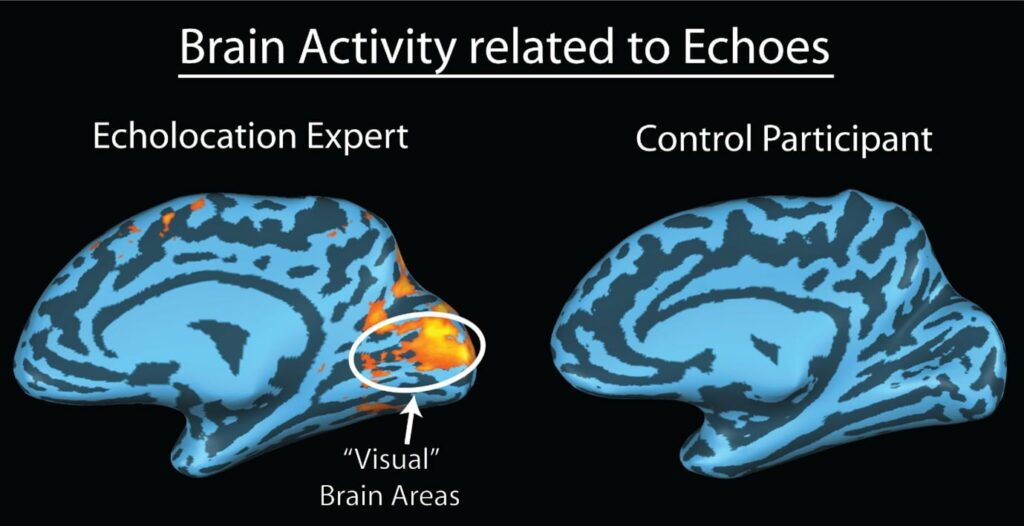
\includegraphics[width=12cm, height=6cm]{Picture-5_Lore-Thaler-min-1024x526.jpg}
        \caption{Imagen de resonancia magnética de actividad eléctrica en el cerebro para ecolocalización humana \cite{humecho}.}
        \end{figure}

\end{frame}

%\begin{frame}

%          \small 
%       \begin{columns}
%          \column{0.45\linewidth}
%            \begin{itemize}
%            %\item 2023 habían reportados 4 millones de robots operando en fabricas.
%            \item El mercado actual de robots es de 1.5 billones de dólares. Se estima que para el 2035 el mercado de robots humanoides alcance los 38 billones de dólares.
%            \item Para que una maquina sea autónoma y se pueda desempeñar con seguridad en múltiples entornos necesita tener una extraordinaria percepción de su ambiente.             
%            \end{itemize}  

%           \column{0.5\linewidth}
%                        \centering
%             \begin{figure}
              %\begin{center}
%                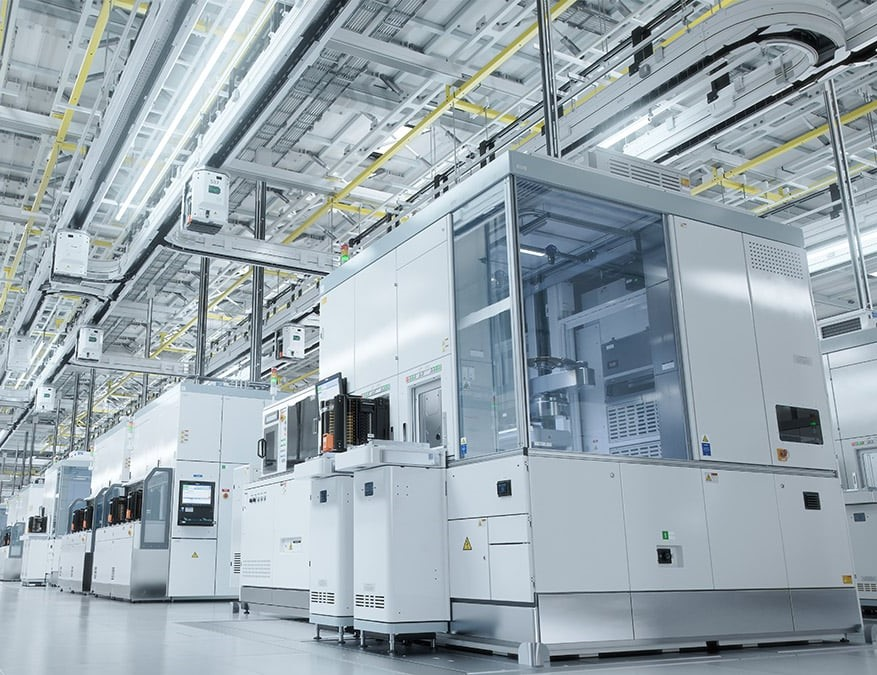
\includegraphics[height=8cm, width=9cm]{semiconductor-manufacturing-facility reduction.jpg}
                %\caption{Proyección global de mercado de robots humanoides hasta el 2035.}
%                \label{fig:gsprojec}
                %\end{center}
%            \end{figure}


%         \end{columns} 
%\end{frame}



%\begin{frame}

%          \small 
%       \begin{columns}
%          \column{0.58\linewidth}
%             \centering
%             \begin{figure}
              %\begin{center}
%                \includegraphics[height=6cm, width=10cm]{GSrobotic projection.png}
%                \caption{Proyección global de mercado de robots humanoides hasta el 2035.}
%                \label{fig:gsprojec}
                %\end{center}
%            \end{figure}
%           \column{0.4\linewidth}
           

%            \begin{itemize}
%            \item En el futuro cercano se tendrá una cantidad considerable robots.
%            \item Percepción de máquina debe ser igual o inclusive superior a la humana.
%            \item Actualmente el estado del arte en percepción de máquina es visual.
%            \item Existe un campo en desarrollo que contempla la percepción acústica de espacios y objetos.            
%            \end{itemize}  
%         \end{columns} 
%\end{frame}




%\begin{frame}{}

%Robots are expected to navigate in multiples and different environments, in order
%to achieve this we need to allow them to have situational awareness and autonomy to
%make proper decisions.\\
%\\
%With visual analysis, the machine can create internal models
%that contain a vast knowledge of the environment, this doesn’t mean that %its
%perception is complete.

%\end{frame}

\begin{frame}
\frametitle{Tabla de Contenidos}
\tableofcontents
\end{frame}


\section{Introducción}
%-------------------------------------------------------------------------

\begin{frame}{Respuesta al Impulso de una Habitación (\textbf{RIH})}


        \begin{itemize}%[<+-|alert@+>]
        %\item Un impulso acústico es un pulso agudo y estrecho cuyo espectro esta compuesto por una distribución uniforme de todas las frecuencias.
        \item El \textbf{RIH} es la función de trasferencia del sonido desde la fuente hasta los receptores.
        \item Es la ``firma'' de la acústica de una habitación. 
        \end{itemize}

        %\uncover<3->{
        \begin{figure}
        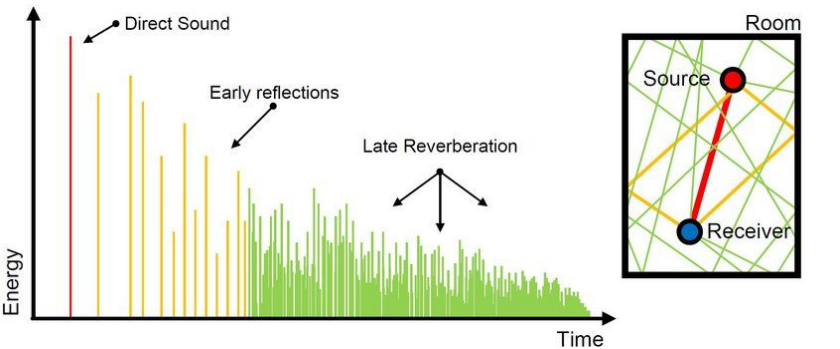
\includegraphics[width=9cm, height=4cm]{RIR.png}
        \caption{\textbf{RIH} y la representación geométrica de una habitación \cite{RIR03}.}
        \end{figure}

\end{frame}

\begin{frame}{\textit{Beamforming}}
    \begin{minipage}{0.45\textwidth}
            
        \begin{itemize}%[<+-|alert@+>]
        \item Técnica de filtrado espacial.
        \item Usa arreglos de micrófonos para combinar señales.
        \item La relación de fase de las señales determina si amplifica o atenúa.
        \end{itemize}
    \end{minipage}
    \begin{minipage}{0.5\textwidth}
        %\uncover<3->{
        \begin{figure}
        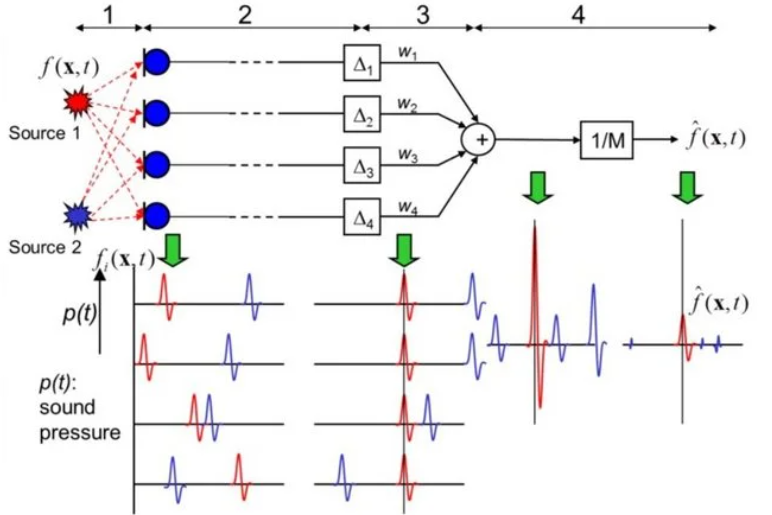
\includegraphics[width=\textwidth, height=5cm]{Beamforming.png}
        \caption{\textit{Beamforming} por retraso y sumatoria \cite{beamf}.}
        \end{figure}
    \end{minipage}
\end{frame}


%\begin{frame}{Red de Estado de Eco (\textit{\textbf{ESN}} por sus siglas en ingles)}

\begin{frame}{\textit{Echo State Network} (\textbf{\textit{ESN}}) }
\small
        \begin{itemize}%[<+-|alert@+>]
        \item \textbf{\textit{ESN}} es una red neuronal recurrente del paradigma de \textit{Reservoir Computing (\textbf{RC})}.
        \item El \textit{reservoir} es la parte recurrente de la red, este transforma secuencias de valores \\ de entrada a estados en un espacio de alta dimensionalidad \footnote{\scriptsize {M. Lukoševičius and H. Jaeger. Reservoir computing approaches to recurrent neural network training. Computer Science Review, 3(3):127–149, 2009.}}.
        \item El \textit{reservoir} es estático, solo la salida de la red es entrenada.
        \item El entrenamiento es sencillo comparado con red recurrente tradicional.
        
        \end{itemize}

        %\uncover<3->{
        \begin{figure}
        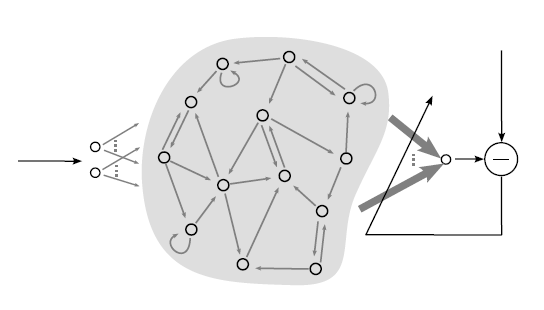
\includegraphics[width=4cm, height=2.5cm]{imgRC1_red.png}
        \caption{\footnotesize Red ESN con su \textit{reservoir} resaltado en gris, las flechas obscuras indican entrenamiento \cite{RC1}.}
        \end{figure}

\end{frame}

\section{Trabajos Relacionados}   
 %-----------------------------------------------------------------------
\begin{frame}{Trabajos Relacionados}

\scriptsize
%\tiny
\begin{table}
\begin{center}
\begin{tabular}{|>{\centering\arraybackslash}m{2cm}|c|>{\centering\arraybackslash}m{6cm}|m{1.4cm}|c|}
    \hline
    Autores & A\~no& Logro & Tipo & Método \\ 
    \hline
     Peters et al.  & 2012 & Identificación de habitaciones mediante sonido \cite{RIR05}. & Clasificación & Aprendizaje automático\\ 
    \hline
    Dokmanić et al. & 2013 & Estimación de la forma de una habitación mediante ecos \cite{RIR07}. & Estimación & Matrices euclidianas\\ 
    \hline
    Brunetto et al. & 2020 & Creación de imágenes de profundidad mediante ecos acústicos \cite{bat1}. & Generativo & Aprendizaje automático\\
    \hline 
    Manabe et al.   & 2022 & Reconocimiento de superficies y bordes de objetos usando ondas estacionarias \cite{shape1}. & Estimación & Espectros de distancia\\
    \hline
    Rothstein et al. & 2023 & Identificación estructuras cerradas desde su interior mediante ecos \cite{echosense}. & Clasificación & Aprendizaje automático\\
    \hline 
    Wang et al.	& 2024 & Detectar, localizar e identificar humanos dentro de habitaciones mediante sonidos \cite{RIR09}.	& Estimación & Aprendizaje automático\\
    \hline
    Bitterman et al. & 2024 & Clasificar habitaciones basado en tamaño y forma mediante RIH \cite{RIR06}. & Clasificación  & Aprendizaje automático\\
    \hline

\end{tabular}
\end{center}
\caption{Trabajos m\'as significativos en percepción acústica de  objetos y espacios.}
\label{table:1}
\end{table}

\end{frame}





\begin{frame}{Características Comunes}
    \begin{minipage}{0.45\textwidth}
            
        \small  
        \begin{itemize}%[<+-|alert@+>]
        \item La mayoría tiene como objetivo la identificación o la clasificación.
        \item Emplean enfoques de aprendizaje de maquina basados en redes \textit{feedforward}.
        \item Por la dificultad de las mediciones acústicas emplean conjuntos de datos pequeños.
        \item Se enfocan en habitaciones grandes.
        \end{itemize}
        
    \end{minipage}
    \begin{minipage}{0.5\textwidth}
        %\uncover<3->{
        \begin{figure}
        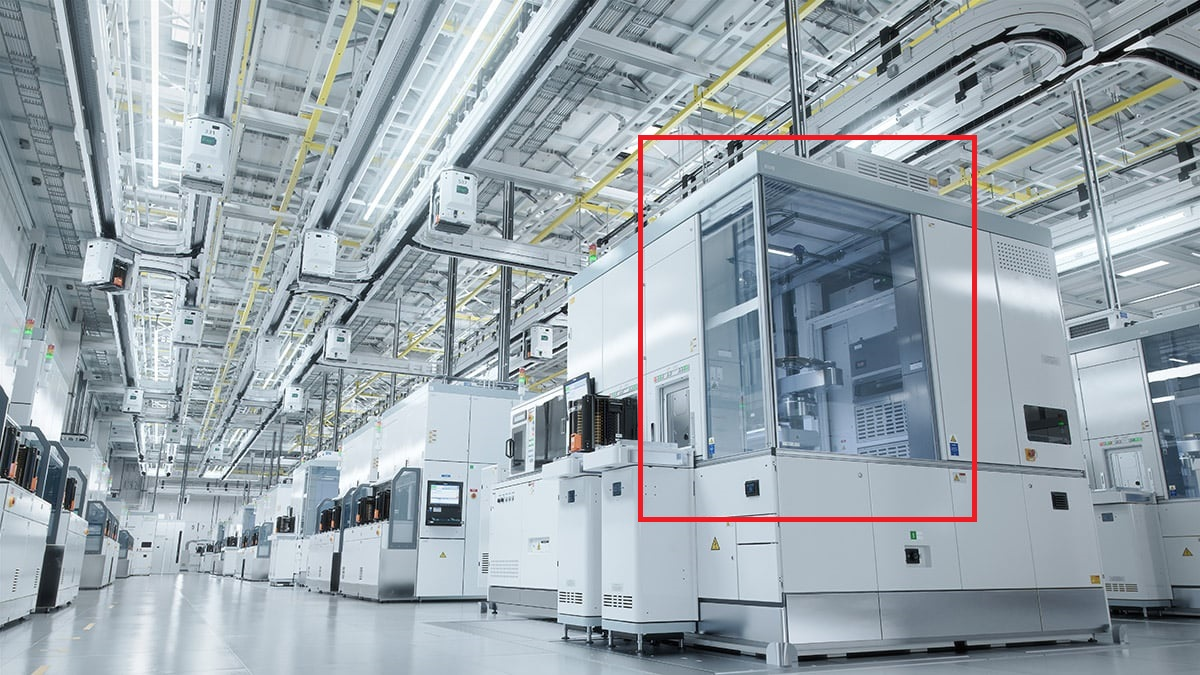
\includegraphics[width=\textwidth, height=5cm]{semiconductor-manufacturing-facility.jpg}
        \caption{Piso de manufactura automatizado para semiconductores.}
        \end{figure}
    \end{minipage}
\end{frame}








\section{Problema y Propuesta de Solución}
%-------------------------------------------------------------------------

\begin{frame}{Problema}
Lo anterior nos lleva a formular el siguiente problema:
\\~\\
\begin{itemize}

    \item Para espacios pequeños (Aprox. 1\(m^3\)) en donde su acústica presenta ecos que llegan de diferentes direcciones al mismo tiempo y se superponen se quiere estimar la posición y orientación de un objeto de interés dentro de ese espacio, esto mediante la respuesta a un impulso acústico.    

        
\end{itemize}

\end{frame}


\begin{frame}{Propuesta de Solución}

    Teniendo como entrada un conjunto de RIH, usar aprendizaje de m\'aquina que transforme estas series acústicas en coordenadas de ubicación y ángulos de orientación de un objeto de interés en su interior.\\  
    Usando:
        \begin{itemize}%[<+-|alert@+>]
        \item \textit{Beamforming} para resolver la superposición de ecos.
        \item Redes neuronales recurrentes en la forma de ESN para procesar directamente las series temporales.
        \end{itemize}
        
\end{frame}

\begin{frame}{Hipótesis}

 ``Una secuencia de procesamiento que emplee \textit{beamforming} y aprendizaje de máquina en la forma de \textit{\textbf{ESN}} puede utilizar la información geométrica que esta comprendida en un conjunto de \textbf{RIH} para inferir o estimar la posición y orientación de un cubo de 20cm de lado ubicado dentro de un espacio pequeño, cuyas dimensiones sean cercanas a un metro \footnote{Basado en las limitaciones encontradas por Brunetto et al. en el sistema de \textit{Batvision} \cite{bat1}.}, esto para cambios de posición no menores a 5cm en alguna de sus coordenada y cambios de orientación mayores a 10 grados, lo anterior con un error de posición menor a 2cm y de orientación menor a 6 grados \footnote{Basado en las dimensiones de deformación detectables por Rothstein et al en su trabajo de \textit{Echosense} \cite{echosense}.}''     


\end{frame}





\section{Objetivos y Metodología}
%-------------------------------------------------------------------------

\begin{frame}{Objetivo General}

Desarrollar y evaluar un sistema por etapas que emplee \textit{beamforming} junto con \textbf{\textit{ESN}} para transformar una entrada multicanal de señales acústicas a coordenadas y ángulos que permitan estimar la ubicación de un objeto en un espacio cerrado. 

\end{frame}


\begin{frame}{Objetivos Específicos}

\begin{itemize}%[<+-|alert@+>]
\item Colectar un conjunto de datos de la respuesta acústica de un espacio pequeño y cerrado para múltiples posiciones de un objeto dentro de este.
\item Desarrollar una etapa de aprendizaje basado en redes neuronales convolucionales (\textit{CNN}) que sea la referencia para estimar coordenadas y orientación de un objeto dentro de un espacio cerrado. 
\item Desarrollar una etapa de aprendizaje que use \textit{ESN} para estimar coordenadas y orientación de un objeto dentro de un espacio cerrado.
\item Implementar un etapa de \textit{beamforming} que permita dividir el espacio en ocho regiones de audición.
\item Evaluar experimentalmente la exactitud y precisión de los estimadores. 


\end{itemize}
\end{frame}

\section{Metodología}

\begin{frame}{Metodología: Caja de Medición}

 \begin{figure}
        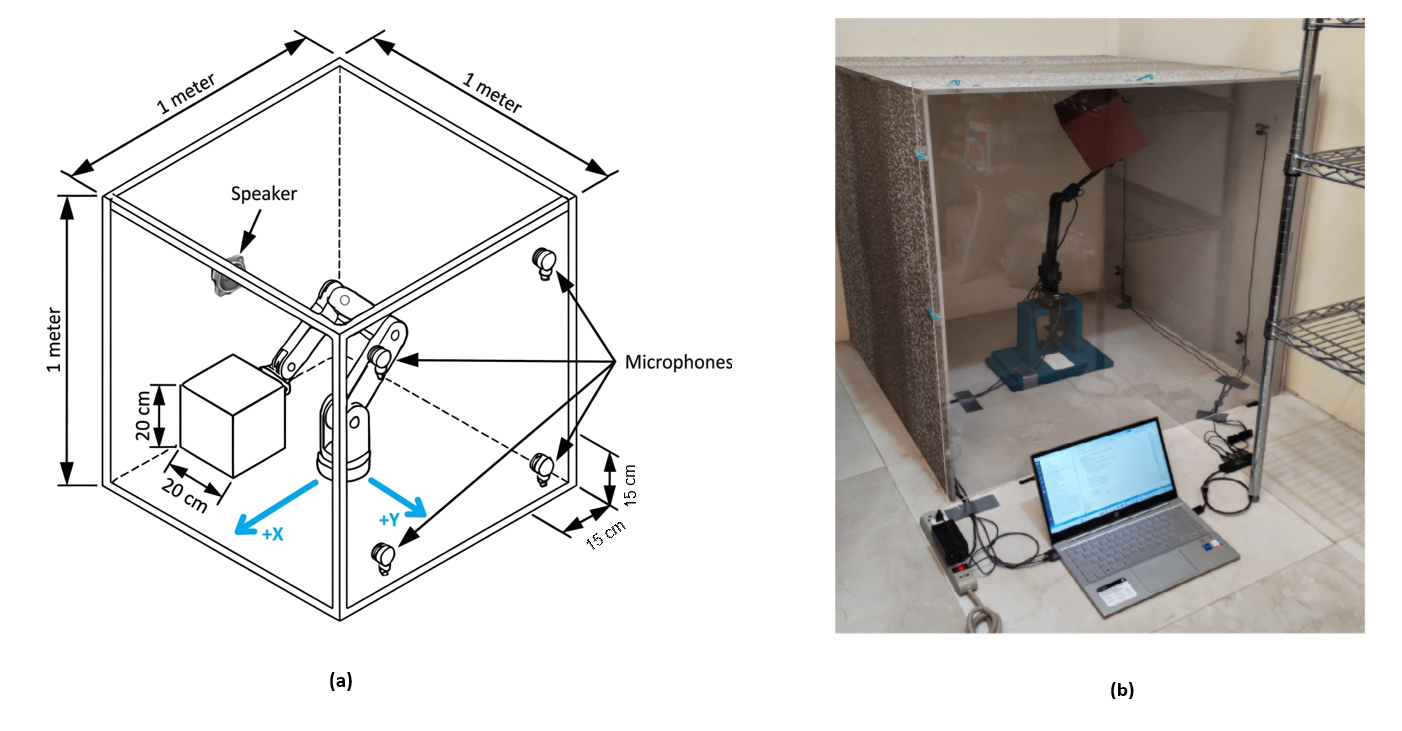
\includegraphics[width=12cm, height=6cm]{Measuretogether.png}
        \caption{Caja de medición: (a) esquema conceptual de la caja para mediciones acústicas y (b) implementación real para la adquisición de datos.}
\end{figure}

\end{frame}


\begin{frame}{Metodología: Recolección de Datos}
    \begin{minipage}{0.5\textwidth}
        \begin{itemize}%[<+-|alert@+>]
        \item La señal era un fragmento de 0,3 segundos de una melodía.
        \item El conjunto de datos se recopiló en 26 sesiones.
        \item Cada sesión consistió en 30 ubicaciones distintas del cubo.
        \item En cada ubicación se registraron nueve orientaciones del cubo.
        \item Por sesión se obtuvieron 270 muestras a cuatro canales cada una.
        \item En total se obtuvieron 7020 muestras a cuatro canales cada una.  
        \end{itemize}
    \end{minipage}
    \begin{minipage}{0.45\textwidth}
        %\uncover<3->{
        \begin{figure}
        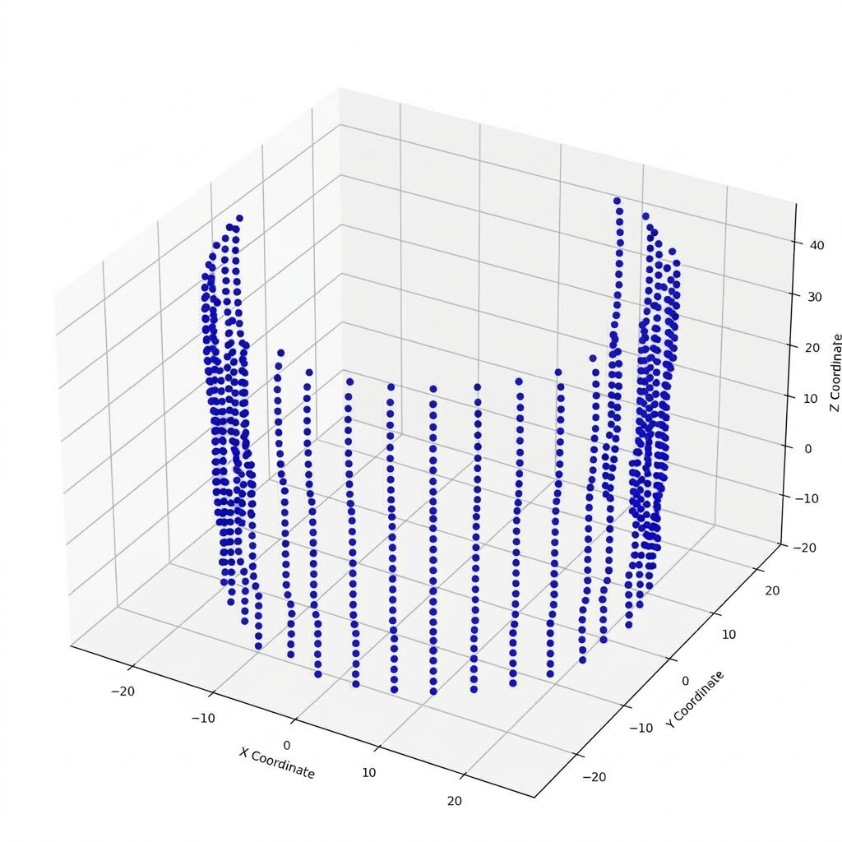
\includegraphics[width=7cm, height=7cm]{allpoints.png}
        \caption{Gráfico de las ubicaciones del cubo para cada grabación del conjunto de datos.}
        \end{figure}
    \end{minipage}
\end{frame}


\begin{frame}{Metodología: Procesamiento de los Datos}

\begin{figure}
        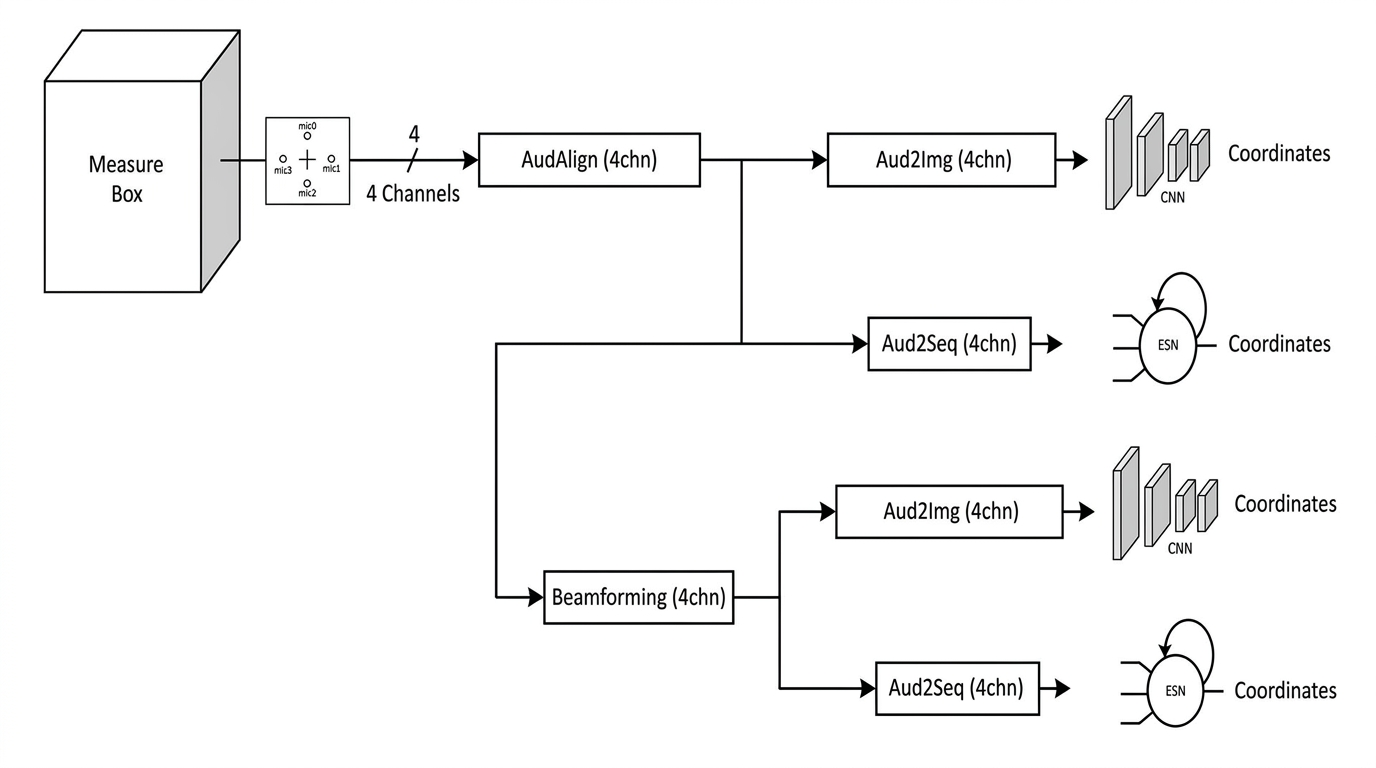
\includegraphics[width=12cm, height=5cm]{AcousticPipeline.jpeg}
        \caption{Diagrama con las etapas de procesamiento de datos de los estimadores.}
\end{figure}

\end{frame}

\begin{frame}{Metodología: Análisis de los Datos}

%    \begin{minipage}{0.5\textwidth}
        \begin{itemize}%[<+-|alert@+>]
        \item Se emplea \textit{five-fold cross-validation} para el entrenamiento y evaluacion de los modelos.
        \item Se evaluan dos métricas: 
        \begin{itemize}
            \item \textit{Mean Absolute Error (MAE)}.
            \item El coeficiente de Pearson.
        \end{itemize}
        \item Se presenta la distribución de los errores de estimación para cada coordenada.
        \item Se comparan los resultados mediante el modelo bayesiano de Plackett-Luce. 
   
        \end{itemize}

\end{frame}

\section{Diseño}   
 %-----------------------------------------------------------------------

\begin{frame}{CNN}

    \vspace*{-0.6cm}

    \begin{minipage}{0.5\textwidth}
        
        \begin{itemize}%[<+-|alert@+>]
            \item Log-Mel spectrogramas como entrada para la CNN.
            \item Arquitectura ResNet-18: $\sim$ 11 millones de parámetros.
            \item La entrada es un stack de 4 imágenes de espectrogramas RGB.
            \item Única salida de regresión con función de activación sigmoidal.
            \item Normalización min-max y arcsin.
            \item Entrenado por 40 épocas: $\sim$1.2 horas.
  
        \end{itemize}
    \end{minipage}
    \begin{minipage}{0.45\textwidth}
        %\uncover<3->{
        \begin{figure}
        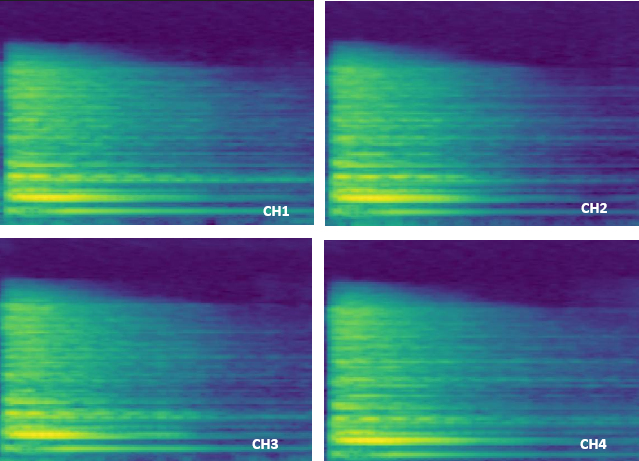
\includegraphics[width=6cm, height=5cm]{4channelSpec.png}
        \caption{Espectrogramas Log-Mel sesión 1, en la ubicación X=22.8 cm, Y=-0.94 cm, Z=-9.43 cm y con una orientación de 50 grados.}
        \end{figure}
    \end{minipage}


\end{frame}

\begin{frame}{ESN}

\begin{columns}[T,onlytextwidth]
    \begin{column}{0.55\textwidth}
        \small
        \begin{itemize}
            \item Secuencia de espectrogramas como entrada para la ESN con 128 features por 40 frames.
            \item Grid search para la optimización de hiperparámetros.
        \end{itemize}

        \begin{table}
            \centering
            \caption{Echo State Network (ESN) Hyperparameters}
            \label{tab:esn_values}
            \scriptsize
            \begin{tabular}{lr}
                \hline
                \textbf{Parameter} & \textbf{Value} \\
                \hline
                Reservoir Size   & 1500 \\
                Spectral Radius  & 0.99 \\
                Sparsity         & 0.1  \\
                Leaky Rate       & 0.1  \\
                Intermediate Captures & 4 \\
                \hline
            \end{tabular}
        \end{table}
    \end{column}
    \begin{column}{0.43\textwidth}
        \begin{figure}
            \centering
            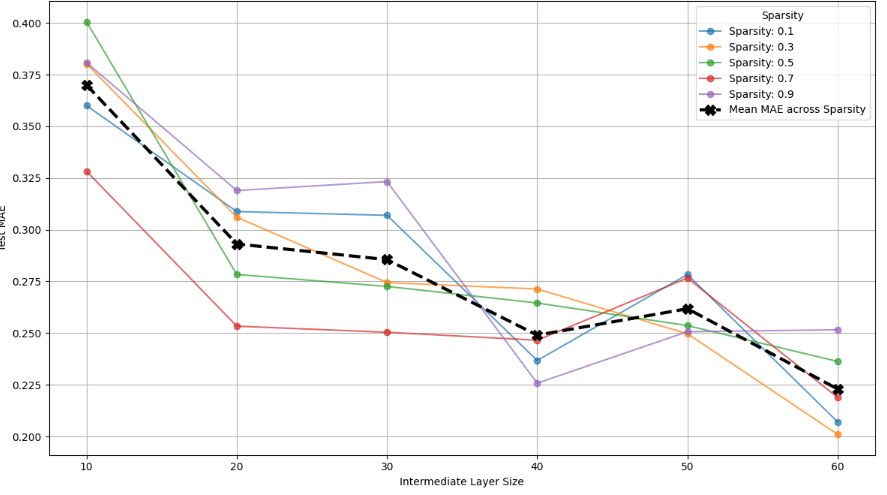
\includegraphics[width=\linewidth,height=4cm,keepaspectratio]{sparcityhiddenlayer.png}
            \caption{\scriptsize MAE en función del tamaño de la capa oculta para distintos valores de \textit{sparsity}.}
        \end{figure}
    \end{column}
\end{columns}

\end{frame}



\begin{frame}{Multihead ESN}

\begin{columns}[T,onlytextwidth]
    \begin{column}{0.50\textwidth}
        \small
        \begin{itemize}
            \item ESN con MAE > 2cm y solamente 62\% de las estimaciones con errores inferiores a $\pm 2$ cm.
            \item Multihead ESN para mejorar la precisión de las estimaciones.
            \item Entrenada cada cabeza de manera independiente, Total $\sim$ 1.5h.
        
        \end{itemize}

    \end{column}
    \begin{column}{0.50\textwidth}
        \begin{figure}
            \centering
            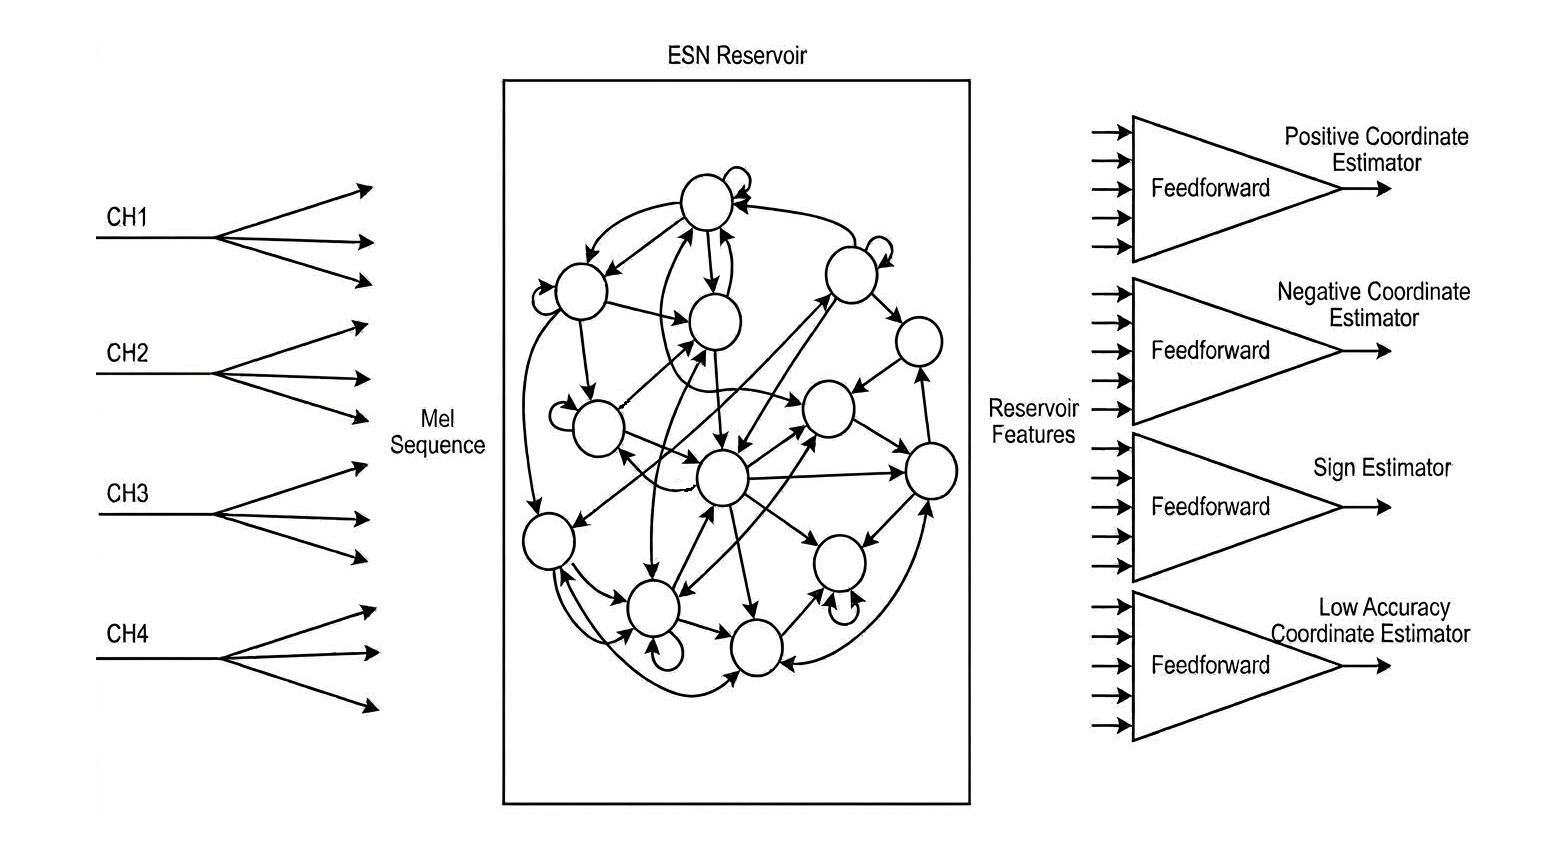
\includegraphics[width=\linewidth,height=4cm,keepaspectratio]{Multi-Head_ESN_Estimator.jpg}
            \caption{\scriptsize Arquitectura de la red multi-cabeza para el estimador ESN.}
        \end{figure}
    \end{column}
\end{columns}


\end{frame}




\begin{frame}{Beamforming}

\vspace*{-0.6cm}

\begin{columns}[T,onlytextwidth]
    \begin{column}{0.50\textwidth}
        \small
        \centering
        \vspace*{1cm}
        \begin{itemize}
            \item Frecuencia minima de operación 123 Hz.
            \item Senal de audio de 10kHz ancho de banda con principales componentes a 400 Hz.
            \item Diferencia en tiempo de llegada entre los micrófonos de 1.34ms a una velocidad de sonido de 343 m/s.
            \item Cuatro pares diferenciales de audio obtenidos como resultado.
        
        \end{itemize}

    \end{column}
    \begin{column}{0.50\textwidth}
        \begin{figure}
            \centering
            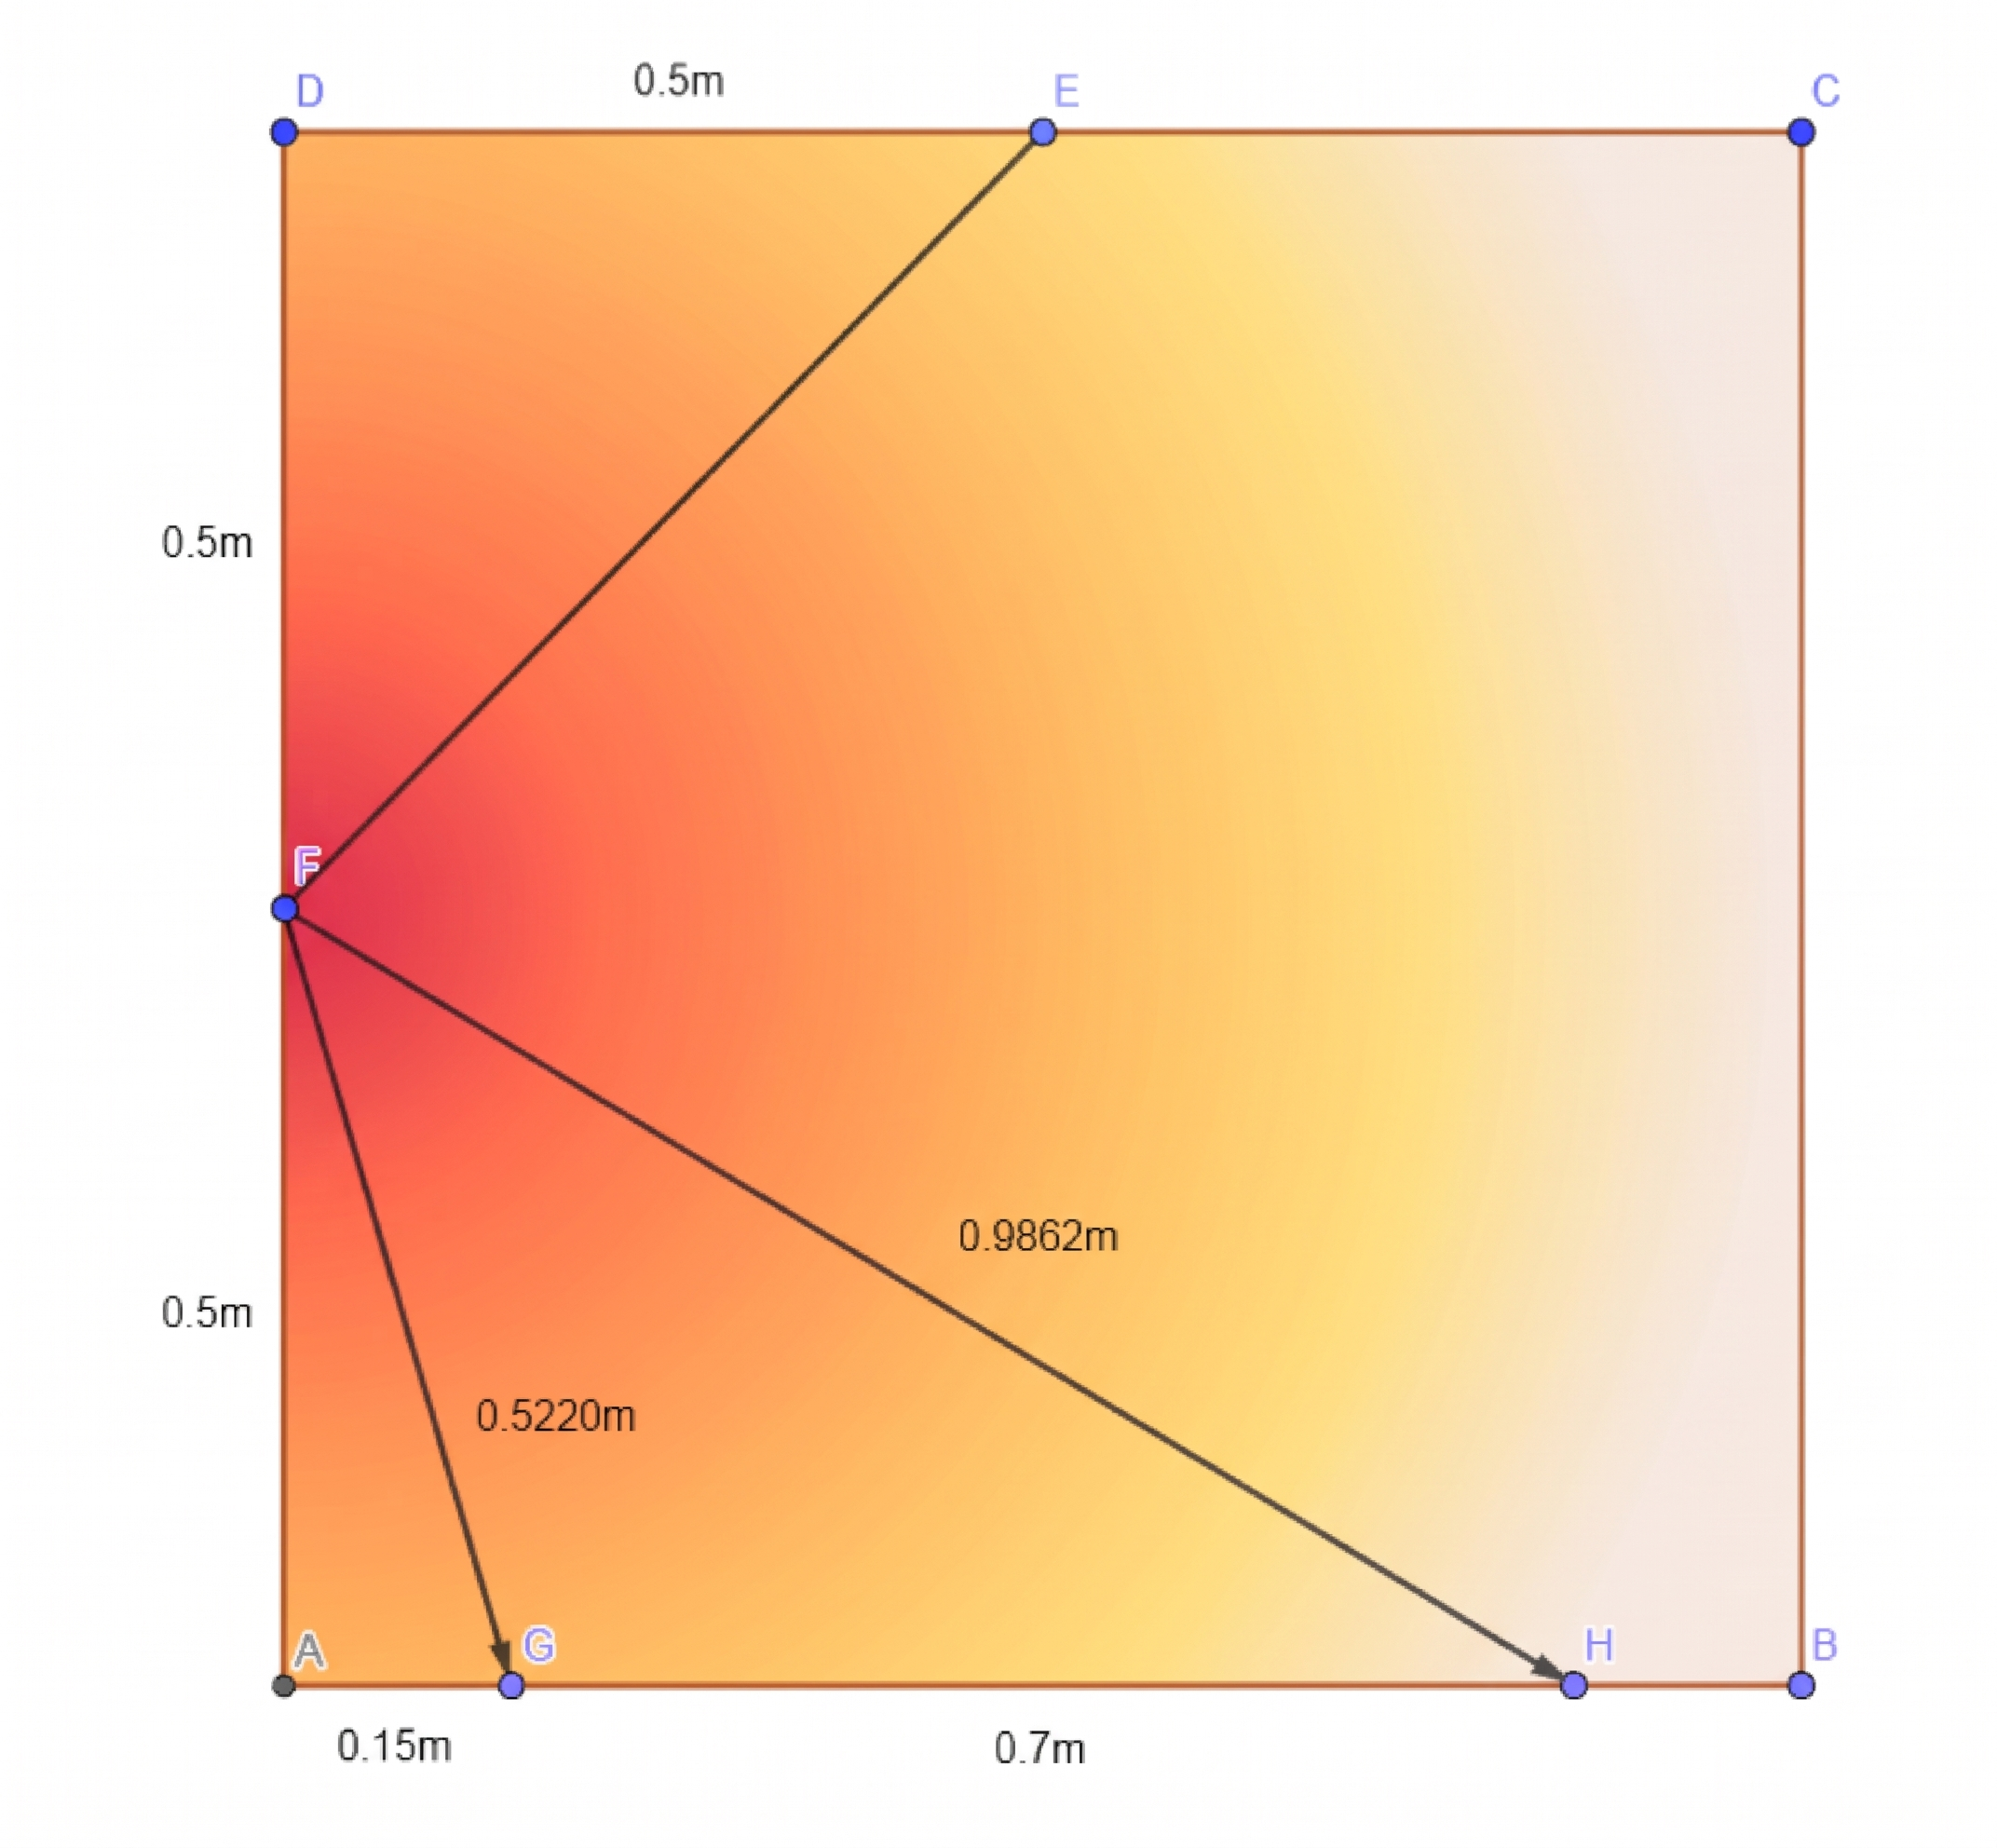
\includegraphics[width=6cm,height=6cm,keepaspectratio]{Beamforming.jpg}
            \caption{\scriptsize Geometric layout of the measurement box illustrating the acoustic path
from the speaker located at E to the microphones positioned at G and H}
        \end{figure}
    \end{column}
\end{columns}


\end{frame}








%\begin{frame}{Escribiendo libremente hacia su tesis}
%    \begin{minipage}{0.5\textwidth}
%        \begin{itemize}%[<+-|alert@+>]
%        \item<.-> \textcolor{myblue} {Escriba lo que sea.}
%        \item<.-> \textcolor{myblue} {Escribir diez minutos al día.}
%        \item<.-> \textcolor{myblue} {Gradualmente aumente la cantidad de tiempo.}
%        \item<.-> \textcolor{myblue} {Escriba sobre un tema.}
%        \item<.-> \textcolor{myblue} {Regrese a sus ideas, repáselas.}
%        \item<.-> \textcolor{myblue} {Permita el pensamiento divergente.}
%        \end{itemize}
%    \end{minipage}
%    \begin{minipage}{0.45\textwidth}
%        %\uncover<3->{
%        \begin{figure}
%        \includegraphics[width=5cm, height=5cm]{BajoUnArbol.JPG}
%        %\caption{here's the image!}
%        \end{figure}
%    \end{minipage}    

%\end{frame}

\section{}

\begin{frame}

Aspectos clave de contribución de la tesis:
\\~\\
          \small 
          \begin{itemize}
          \item Demostraría que es posible localizar y determinar la orientación de un objeto en un espacio pequeño.
          \item Demostraría que \textit{beamforming} es una opción para solucionar el problema de \\ superposición de ecos en espacios pequeños.
          \item Indicaría que ESN es mejor que CNN para análisis de ecos acústicos.
          \end{itemize}
%       \begin{columns}
%          \column{0.45\linewidth}
%            \begin{itemize}
%            %\item 2023 habían reportados 4 millones de robots operando en fabricas.
%Basado en una proyección de Morgan Stanley, se estima que para el 2050 el mercado de robots humanoides alcance los 5 trillones.
%Para que una maquina sea autónoma y se pueda desempeñar con seguridad en múltiples entornos necesita tener una extraordinaria percepción de su ambiente.             

\end{frame}

\begin{frame}{}
        \begin{figure}
        \includegraphics[width=6cm, height=5cm]{gracias}
        %\caption{here's the image!}
        \end{figure}
\end{frame}

\begin{frame}[allowframebreaks]
        \frametitle{Referencias}
        \bibliographystyle{ieeetr}
        \bibliography{mendeley}
\end{frame}
    
\end{document}